%Andrea

In questa lezione si svilupperanno tre ``tipi'' di teoremi di trasversalità. Non verrà data una dimostrazione degli stessi, né ora, né durante il corso, tranne qualche idea.

\begin{description}
\item [Tipo 1] %"Se $f$ è trasversa allora la situazione è "semplice""
\begin{teo}[Teorema 1]
Siano $X$ e $Y$ varietà differenziabili, $A\subseteq Y$ e $\fundef[f]{X}{Y}$  tale che $f\pitchfork A$. Allora $f^{-1}(A)$ è una sottovarietà di $X$.
\end{teo}
\item [Tipo 2] %"le funzioni trasverse sono ovunque..."
\begin{teo}[Teorema 2]
Le funzioni trasverse ad $A\subseteq Y$ sono un aperto denso in $\mathcal E(X,Y)$.
\end{teo}
\begin{teo}[Teorema 2++] \footnotemark %"E ti omotopano la vita"\\
Sia $f \not\pitchfork A$. Esiste una funzione $g$ arbitrariamente vicina a $f$ tale che $g\pitchfork A$. Se $X$ non è chiusa ed $f|_{\partial X} \pitchfork A$ puoi scegliere $g$ tale che coincida con $f$ in un collare del bordo di $X$.
\end{teo}
\marginpar{Ma la prima affermazione di questo teorema non è già nel teorema 2 quando si afferma che l'insieme è un aperto \emph{denso}}
\item [Tipo 3] %"Siano pure trasverse, ma che siano almeno cobordanti!"
\begin{teo}[Teorema 3]
Siano $X_1$ e $X_2$ varietà compatte e senza bordo della stessa dimensione, $Y$ varietà e $A$ sottovarietà di $Y$. Siano inoltre $\fundef[f_1]{X_1}{Y}$ e $\fundef[f_2]{X_2}{Y}$. Se $f_1 \pitchfork A$ e $(X_1,f_1) \sim_{cob} (X_2,f_2)$ detti $Z_1=f_1^{-1}(A)$ e $Z_2=f_2^{-1}(A)$ si ha che $(Z_1, f_1|_{Z_1}) \sim_{cob} (Z_2,f_2|_{Z_2})$.
\end{teo}
\marginpar{Inserirò un bel disegno quando imparerò a farlo!!!}
\begin{proof}
 Diamo un po' di idee per la dimostrazione, dando per noti gli altri teoremi già esposti. Per il teorema~1 $Z_1$ e $Z_2$ sono delle sottovarietà di $X_1$ e di $X_2$. Chiamiamo $W$ la varietà che realizza il cobordismo ($\boundary W = X_1 \sqcup X_2$) ed $F$ la relativa funzione ($F|_{X_1} = f_1$ e $F|_{X_2}=f_2$). Grazie al teorema~2 esiste una funzione $\fundef[G]{W}{Y}$ vicina a piacere ad $F$, che ristretta su $\boundary W$ valga $f_1\sqcup f_2$ (anzi, il teorema ci garantisce che la possiamo scegliere in modo che coincida con $F$ in un collare di $X_1\sqcup X_2$) e che sia trasversa ad $A$. Chiaramente la controimmagine di $G$ in $W$ è una sottovarietà per il teorema~1 e, grazie al fatto che $G$ coincide con $F$ in un collare di $X_1 \sqcup X_2$ ne segue che $G|_{G^{-1}(A)}$ realizza il cobordismo fra $Z_1$ e $Z_2$.
 \end{proof}
\end{description}

Vediamo ora qualche semplice applicazione della teoria della trasversalità.
Perdonatemi per quello che sto per fare.

\begin{defn}[Retrazione]
Sia $X$ una varietà con bordo. $\fundef[\tau]{X}{\boundary X}$, liscia, è una retrazione se $\tau|_{\boundary X}=\id_{\boundary X}$.
\marginpar{Penso debba essere una funzione liscia, perchè di funzioni arbitrarie ne trovi a pacchi (Ale)}
\marginpar{Devo ancora inserire qualche disegnino qui}
\end{defn}

\begin{teo}
Non esistono retrazioni!
\end{teo}
\begin{proof}
Procediamo per assurdo. Sia $y_0 \in \boundary X$. Prendo $\tau$ retrazione. Prendo una funzione $\tau'$ vicina a piacere a $\tau$ che coincida con $\tau$ sul bordo e trasversa ad $\{y_0\}$. Considero $Y=\tau'^{-1}(y_0)$. $Y$ è una varietà 1-dimensionale, per il teorema 1 di trasversalità, e $y_0\in Y$. Dunque $Y$ ha bordo non vuoto. Ma, per la caratterizzazzione delle varietà 1-dimensionali deve avere almeno un altro punto $y_1$ nel bordo. Dunque $y_1=\tau(y_1)=\tau'(y_1)=y_0$. Assurdo.  
\end{proof}
Forse potreste perdonarmi grazie a questo:
\begin{teo}[Teorema del punto fisso di Brouwer]
Sia $D^n$ il disco chiuso di raggio~1 in $\R^n$. Sia $\fundef[f]{D^n}{D^n}$. Esiste $x_0\in D^n$ punto fisso per $f$.
\end{teo}
\begin{proof}
Per assurdo non vi sia alcun punto fisso per $f$. Sia $\fundef[r]{D^n}{\boundary D^n}$ tale che $r(x)$ sia l'intersezione di $\boundary D^n$ con la semiretta di origine $f(x_0)$ passante per $x_0$. $r$ è una retrazione. 
\end{proof}

\begin{center}
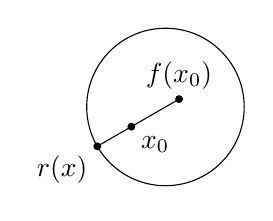
\begin{tikzpicture}
\pgfmathsetmacro\angle{30}
\draw (0,0) circle (1);
\draw (\angle:.2) coordinate (fxzero) -- (\angle:-1) coordinate (rx);
\fill (fxzero)      circle (.05) node[above]       {$f(x_0)$};
\fill (\angle:-0.5) circle (.05) node[below right] {$x_0$};
\fill (rx)          circle (.05) node[below left]  {$r(x)$};
\end{tikzpicture}
\end{center}




